\documentclass[11pt, a4paper, french, openright]{report}
% version reliée
% \documentclass[11pt, a4paper, french, openright, twoside]{report}
\usepackage[french]{babel}
\selectlanguage{french}
\usepackage[T1]{fontenc}
\usepackage[utf8]{inputenc}
\usepackage{lmodern,textcomp}
\usepackage[
    left = \flqq,%
    right = \frqq,%
    leftsub = \flqq,%
    rightsub = \frqq%
]{dirtytalk}

\usepackage{csquotes}
\usepackage{hyperref}

\usepackage{graphicx}
\usepackage{caption}
\usepackage{setspace}

\usepackage{titling}

\usepackage[backend=biber]{biblatex}
\bibliography{bibliography}

\newcommand{\HRule}{\rule{\linewidth}{0.5mm}}
\renewcommand{\thefootnote}{\alph{footnote}}

\title{Comment devenir leader de son marché en quelques années et en partant de zéro}

\author{Axel Leroy}

\date{\today}

\begin{document}

\begin{titlepage}
\begin{center}

% Upper part of the page. The '~' is needed because only works if a paragraph has started.

\includegraphics[width=0.35\textwidth]{./ParisOuest}~\\[1cm]

\textsc{\LARGE Université Paris Ouest La Défense}\\[1.5cm]

\textsc{\Large }\\[0.5cm]

% Title
\HRule

{\huge \bfseries \thetitle \\[0.4cm] }
{\Large \bfseries Par l'étude des cas Netflix, SpaceX, Spotify et Tesla Motors \\[0.4cm]}

\HRule

\vspace{5mm}

% Author and supervisor
\begin{minipage}{0.4\textwidth}
\begin{flushleft} \large
\emph{Auteur:}\\
Axel \textsc{Leroy}
\end{flushleft}
\end{minipage}
\begin{minipage}{0.4\textwidth}
\begin{flushright} \large
\emph{Tuteurs entreprise :} \\
Yannick \textsc{Ameur}\\
Nathaniel \textsc{Richand}\\
\emph{Référent:} \\
Sonia \textsc{Guehis}
\end{flushright}
\end{minipage}

\vfill

% Bottom of the page
{\large \today}

\end{center}
\end{titlepage}

%page blanche
\newpage
~
%ne pas numéroter cette page
\thispagestyle{empty}
\newpage

%ne pas numéroter cette page
\thispagestyle{empty}
\begin{center}
\subsection*{Remerciements}
\end{center}

\hskip7mm

\begin{spacing}{1.3}
Je tiens tout particulièrement à remercier Nathaniel {Richand} pour ses conseils et remarques qui m'ont guidé et m'ont été d'une très grande aide durant la rédaction de ce mémoire.

Je souhaite aussi remercier Sonia Guehis d'avoir suivi mon mémoire et Lom Hillah qui a toujours été un grand partisan de l'entrepreneuriat au sein de l'équipe pédagogique.

Enfin je remercie mon tuteur Yannick Ameur, mes collègues Luc Bizeul et Nicolas Montens ; mes équipiers de MIAGE Connection et MIAGE Entrepreneurs et mes amis pour leurs retours et leur soutien. 
\end{spacing}

\newpage
%ne pas numéroter cette page
\thispagestyle{empty}
\newpage

%ne pas numéroter cette page
\thispagestyle{empty}
\begin{abstract}
\hskip7mm

\begin{spacing}{1.3}

L'actualité de ce début d'année a été marqué par les réussites d'entreprises telles que Netflix, SpaceX, Spotify et Tesla Motors. 

Ces entreprises ont toutes moins de vingt ans d'existence et après avoir connu une croissance insolente, s'attaquent désormais aux géants de leurs industries.

Ce mémoire étudie l'origine de cette croissance en s'intéressant à l'élément qui les différencie de ces géants : elles sont en rupture totale dans leurs stratégies et le développement de leurs cultures d'entreprise.

\end{spacing}
\end{abstract}

\tableofcontents
\thispagestyle{empty}
\setcounter{page}{0}
%ne pas numéroter le sommaire

\newpage
~
\thispagestyle{empty}
%recommencer la numérotation des pages à "1"
\setcounter{page}{0}
\newpage

\chapter{Introduction}

Alors que j'ai toujours été fasciné par l'entrepreneuriat et l'innovation qui en découle, ce début d'année 2016 a été marqué par la concrétisation des efforts de plusieurs entreprises clés, ce qui confirme mon sentiment que ces entreprises innovantes changent notre monde :

\vspace{5mm}

L'entreprise \textbf{SpaceX} a réussi le 27 mai dernier à récupérer le premier étage de sa fusée Falcon 9 pour la troisième fois consécutive\supercite{SpaceXThirdLanding} et a ainsi confirmé la viabilité de son projet de fusées réutilisables. Ce après avoir rendu l'exploration spatiale abordable, créé un marché pour l'envoi de charge de poids réduit et être devenue la première entreprise privée à ravitailler la Station Spatiale Internationale le 25 mai 2012\supercite{DragonFirstISSMission}. Pourtant cette entreprise qui souhaite réaliser des voyages habités sur Mars d'ici 2025\supercite{ElonMuskMars2020} n'avait aucune expérience dans le domaine aérospatial lors de sa création en 2002.

\vspace{5mm}

Le 10 février \textbf{Tesla Motors} annonce avoir écoulé 107 000 exemplaires de leurs modèles de voitures électriques S et X en trois ans et demi\supercite{Tesla2015FullYearUpdate}. L'entreprise  qui a commencé avec des passionnés d’électronique rêvant de changer le monde a par la suite dévoilé le 31 mars son quatrième modèle ---le bien nommé \textit{Model 3}. Ce modèle destiné à démocratiser les véhicules électriques auprès des classes moyennes cumulait au 4 mai près de 325 000 de réservations\supercite{Tesla2016Q1Update}, pour une livraison fin 2017 en Amérique du Nord.

\vspace{5mm}

Les 11 et 12 avril \textit{Reed Hastings} présentait la stratégie de sa société \textbf{Netflix} pour les années à venir à la Cité du Cinéma, renommée \textit{Netflix City} pour l'occasion. Le symbole est fort et à l'image des changements que le service a apporté à l'industrie du divertissement et à notre manière de consommer les films et séries. Tout d'abord créé suite au mécontentement de son créateur à l'égard du service de location de films Blockbuster, alors en position de monopole, il a su se faire une place et créer par la suite un nouveau marché avec son service de vidéo à la demande.

\vspace{5mm}

\textbf{Spotify} quant à eux ont annoncé des revenus records de 1,95 milliards d'euros pour l'année 2015 \supercite{SpotifyChiffres2015}. Créé sur le postulat qu'il fallait proposer un service légal qui soit plus pratique que le téléchargement illégal dans une Suède qui avait alors les yeux braqués sur le procès \textit{The Pirate Bay}, le service a su détourner une génération entière du téléchargement illégal et générer plus de revenus que la vente de disques et le téléchargement légal.

\vspace{5mm}

Ces entreprises ont la particularité d'avoir moins d'une vingtaine d'années d'existence et alors qu'elles n'avaient aucune expérience dans leurs domaines respectifs, ont su devenir pionnières de leurs marchés respectifs et sont allés jusqu'à entrer en compétition avec des acteurs historiques.

\textbf{Elles ont pour point commun d'être en rupture totale avec leurs marchés respectifs tout comme sur leurs manières de développer leurs cultures d'entreprise.}

\chapter{Contexte}

Afin de mettre en contexte la réussite des entreprises étudiées, nous allons nous pencher sur l'état de leurs marchés respectifs avant leur création durant le début des années 2000.

\section{Un marché de la location de films dominé par Blockbuster}

Sur le marché américain l'entreprise \textit{Blockbuster} fait figure de poids lourd dans le marché de la location de films depuis près de quinze ans mais se voit concurrencé par la jeune société \textit{Netflix} qui ---contrairement à Blockbuster--- n'impose pas de délais de retour pour les DVD et ne possède aucune boutique physique. 

\section{Une industrie aérospatiale au point mort depuis la fin de la Guerre Froide}

La chute de l'\textit{URSS} en 1991 a marqué la fin de la Guerre Froide et des ambitions de conquête spatiale des États-Unis : bien que la \textit{NASA} a lancé le programme de la \textit{Station Spatiale Internationale} dès 1993, elle ne souhaite plus réaliser de missions spatiales habitées au-delà de la stratosphère, et ce par manque de budget alloué par le Congrès américain. 

De plus le marché de l'envoi de satellites est restreint à une poignée d'entreprises et d'organisations en position de monopole : le français \textit{Arianespace}, les américains \textit{Lockheed Martin Space Systems} et \textit{Boeing} et le russe \textit{RSC Energia} qui pratiquent des prix dissuasifs pour les petites entreprises et organisations.

\section{Des véhicules électriques qui manquent d'autonomie}

On peut difficilement parler d'une industrie tant elle est à ses balbutiements : les principaux constructeurs automobiles ne daignent pas s'intéresser à la création de véhicules électriques\footnote{Exception faite de \textit{Nissan} qui a produit la \textit{Hypermini} ---produite de 1999 à 2001 et disposant d'une autonomie de 115 kilomètres--- destinée uniquement au marché nippon et la \textit{Altra EV} ---une conversion de la \textit{R'nessa} produite de 1997 à 2001 et disposant d'une autonomie de 230 kilomètres--- qui est restée confiné à un programme pilote comprenant 200 exemplaires. Nissan attendra 2010 pour rentrer à nouveau dans le marché avec sa \textit{Leaf}.} et seuls une poignée de groupes d'étudiants et quelques entreprises de taille mineure ont exploré la création de véhicules entièrement électriques.

Ils se heurtent cependant à un problème majeur : les technologies de batteries de l'époque ne permettent pas de proposer une autonomie décente.

\section{Un marché de la musique cannibalisé par le téléchargement illégal}

Après avoir culminé à 38 milliards de dollars en 1999\supercite{IFPI2000Report}, les revenus de l'industrie de la musique n'ont cessé de chuter jusqu'à atteindre les 18 milliards de dollars en 2008\supercite{IFPI2008Report}. L'industrie accuse alors le téléchargement illégal d'en être à la cause et attaque en justice l'entreprise éditant le logiciel \textit{Napster} en 2000 et la plate-forme de recherche BitTorrent \textit{The Pirate Bay} en 2006, forçant l'un à fermer et l'autre à fuir continuellement les autorités. 

\textit{iTunes} ---la boutique de musique dématérialisée d'Apple--- bien qu'ayant apporté la possibilité d'acheter les titres à l'unité, ne permet cependant pas à l'industrie de combler la chute des ventes de disques. Les principales maisons de disque sont alors désespérées.

\chapter{Des stratégies en rupture avec le marché existant}

\section{Rendre l'exploration spatiale abordable}

Après avoir été écarté de la direction de \textit{X.com} ---l'entreprise qu'il a co-fondé dans l'espoir de révolutionner les paiements en ligne et qui deviendra plus tard \textit{PayPal}--- \textit{Elon Musk} se met en tête de réaliser un de ses rêves de toujours : \textbf{coloniser Mars}.

Après s'être aperçu avec le plus grand désarroi que la conquête de la planète rouge n'était pas à l'agenda de la NASA, il rejoint la \textit{Mars Society}, une organisation à but non-lucratif qui promeut l'exploration et la colonisation de la planète. Dès lors il affiche son souhait de participer à cette aventure en \textbf{lançant lui-même une campagne d'exploration spatiale}, un projet que de nombreux millionnaires avant lui ont entreprit avant d'échouer ou d'abandonner.

Il se tourne d'abord vers des fournisseurs russes dans l'espoir de racheter et réhabiliter des missiles intercontinentaux de l'ex-URSS, mais ces derniers étant trop chers à son goût, \textbf{il décide de créer ses propres fusées}.

\vspace{5mm}

Sa stratégie est alors très claire : alors que \textbf{la technologie des fusées n'a pas évolué depuis près de cinquante ans} et que le \textbf{marché est concentré autour de peu d'acteurs} s'entêtant à créer des fusées excessivement puissantes et chères, son objectif est de capitaliser sur les avancées de la recherche sur les matériaux et les simulations physiques afin de \textbf{produire des fusées abordables capables d'emporter de petites charges} tout en évitant un maximum de gâchis.

Avec cette stratégie, il souhaite ainsi \textbf{relancer l'intérêt pour la conquête spatiale en la rendant plus abordable}, et par la même occasion \textbf{explorer le marché encore délaissé de l'envoi de petites charges} à peu de frais.

Il s'entoure alors de \textit{Tom Hueller}, un ingénieur spécialisé dans les moteurs de fusées depuis près de vingt ans ; et \textit{Chris Thompson}, qui géra la production des fusées Delta et Titan chez Boing. Il fonde \textit{Space Exploration Technologies} ---souvent désigné sous le nom \textbf{SpaceX}--- en Juin 2002 et lance le développement de la fusée \textbf{Falcon 1}, une fusée à deux étages capable d'emporter une charge pouvant aller jusqu'à 670 kg.

\vspace{5mm}

La tâche se révèle cependant difficile, d'autant plus que le planning prévu par Elon Musk était très optimiste. Après trois essais ratés, \textbf{SpaceX réussira à envoyer leur première charge en orbite le 28 septembre 2008}.

\vspace{5mm}

Dès lors l'entreprise va réaliser des \textbf{lancements réguliers afin de s'assurer une indépendance financière} et commence à s'intéresser aux marchés plus importants avec des fusées de plus grandes capacités : la fusée \textbf{Flacon 5} dont le premier étage devait posséder 5 moteurs et capable d'emporter jusqu'à 4100 kg, rapidement abandonnée au profit de la fusée \textbf{Falcon 9} et du vaisseau \textbf{Dragon} développés conjointement dans l'objectif de remplacer la navette spatiale américaine et ainsi profiter du juteux contrat de ravitaillement de la Station Spatiale Internationale.

\vspace{5mm}

Alors que les principaux constructeurs de fusées se contentaient de laisser les différents étages de leurs fusées se noyer dans l'océan et de reconstruire une nouvelle fusée pour chaque lancement, Musk ambitionne de rendre le premier étage de cette nouvelle \textbf{fusée réutilisable dans un esprit de diminuer encore et toujours les coûts}\supercite{MuskAmbitionReusableFalcon9}.

\textbf{L'économie envisagée est alors de 30\%} puisque la remise en état et le carburant ne coûteraient que 4 millions de dollars alors que le premier étage coûte 60 millions de dollars à construire\supercite{SpaceXReusable30Percent}.

\section{Une voiture électrique pour tous}

\textit{Martin Eberhard} et \textit{Marc Tarpenning} sont deux ingénieurs en électronique qui ont créé la technologie des premiers livres électroniques. Après le rachat de leur entreprise, Eberhard commence à chercher une alternative à l'essence et après avoir étudié les piles à combustible, il se tourne vers \textbf{les batteries Lithium-Ion qui ont réalisé des progrès important en terme de capacité} en ce début de vingt-et-unième siècle.

Il se met alors à \textbf{étudier le marché}, réalise des calculs et décide de réaliser une voiture de sport haut-de-gamme, légère et électrique basée sur le châssis d'une Lotus Elise et \textbf{visant les millionnaires souhaitant s'afficher au volant d'une voiture rapide et écologique}.

Il fait également le choix de vendre les voitures directement par Internet et des agences luxueuses dans les centres commerciaux puisqu'ils n'ont pas besoin d'avoir des centaines de concessions, les véhicules électriques nécessitant peu d'entretien.

\vspace{5mm}

Avec Tarpenning ils fondent \textbf{Tesla Motors} en Janvier 2004 et cherchent à lever 7 millions de dollars. Ils rencontrent \textit{Elon Musk} ---qui a reçu 165 millions de dollars suite au rachat de Paypal par eBay--- qui désire changer la dépendance de la société au pétrole avec des véhicules électriques depuis le lycée. \textbf{Il investira 6,5 millions de dollars}, permettant ainsi à Tesla Motors de débuter la conception de leur premier modèle, la \textbf{Tesla Roadster}. Prévu pour début 2006 au prix de 90 000 dollars, il est doté d'une autonomie de 250 milles, une première.

Après plusieurs retards, problèmes de production, réorganisations internes et être passé non loin de la faillite, \textbf{le premier exemplaire de la Roadster sortira des chaînes de production en Février 2008}.

\vspace{5mm}

L'arrivée de liquidités et de nouveaux investisseurs permettra à Tesla de passer à la seconde phase de son plan\supercite{TeslaSecretMasterPlan} et de commencer le développement d'\textbf{une berline de luxe visant les familles aisées et prescriptrices} : la Model S, dont les premiers modèles seront livrés en Juin 2012.

Alors que le Roadster était avant tout une preuve de concept basé sur un châssis existant et assemblé par Lotus\supercite{LotusPosition}, \textbf{ce nouveau modèle serait entièrement conçu et assemblé par Tesla} ---du châssis à la carrosserie--- dans une nouvelle usine à Fremont, Californie.

Cette dernière est rachetée en 2010 à \textit{NUMMI} ---une co-entreprise de \textit{General Motors} et \textit{Toyota} qui n'a pas survécu aux difficultés du marché automobile américain suite à la crise économique de 2008--- et \textbf{est entièrement réorganisée sur le modèle de l'usine SpaceX} avec des chaînes automatisées.

\vspace{5mm}

Le Model S est devenu en très peu de temps \textbf{une icône des véhicules électriques} et est même parvenu à devenir \textbf{le véhicule de luxe le plus vendu} aux États-Unis\supercite{Tesla2015FullYearUpdate} et en Europe\supercite{ModelSLuxuryCarEurope} en 2015.

Bien évidemment, Tesla n'a pas uniquement compté sur son arrivée anticipé sur le marché des véhicules électriques pour arriver à ces résultats : \textbf{la communication est très centrée autour de la sécurité} ---la Model S fait partie des rares voitures à avoir cinq étoiles aux tests de sécurité routière américain \textit{NHTSA} et européen \textit{NCAP}\supercite{ModelSNCAP}---, l'entreprise allant jusqu'à rappeler des milliers de modèles présentant un défaut\supercite{ModelSPartialRecall}, à proposer la pose gratuite d'un bouclier en titane pour protéger les batteries\supercite{ModelSTitaniumShield} et à communiquer sur divers incidents mitigés par la conception de la voiture\supercite{ModelSFire}\supercite{ModelSAccident}.

\vspace{5mm}

Avant même que le Model S sorte ---une habitude de Musk--- Tesla annonce le 9 février 2012 \textbf{un nouveau modèle encore plus attrayant pour les familles} : le Model X, un monospace-SUV de luxe \textbf{basé sur le châssis du Model S} capable de transporter jusqu'à 7 adultes grâce à la place gagnée par l'absence d'un moteur thermique et la présence de portes « \textit{Falcon Wing} » permettant de pouvoir s'asseoir aisément dans la troisième rangée de siège. Les premiers modèles ont été livrés en Amérique du Nord en Septembre 2015 tandis que les livraisons européennes débutent en Juin 2016.

\section{Un service plus pratique que le téléchargement illégal}

Été 2006 en Suède, tous les regards sont tournés vers le procès qui oppose \textit{The Pirate Bay} à l'industrie de la musique. À ce même moment, \textit{Daniel Ek}, jeune entrepreneur et président de \textit{uTorrent} ---l'entreprise éditant l'un des principaux clients BitTorrent, protocole utilisé par The Pirate Bay pour mettre à disposition des fichiers soumis au droit d'auteur---, \textbf{souhaite réaliser un service aussi pratique que \textit{Napster}} ---service qu'il utilisait adolescent et qui a fermé suite au procès subit en 2000--- mais ayant \textbf{un business model viable et capable de rémunérer les artistes}. 

Pour Ek, \textbf{le téléchargement illégal est compliqué} : trouver le titre qu'on souhaite est pénible, le téléchargement dure plusieurs minutes et il faut s'inquiéter des virus informatiques. On ne télécharge non pas par choix, mais par nécessité et Ek est convaincu que si un service est plus pratique et propose une meilleure expérience que le piratage, alors \textbf{les utilisateurs seront prêts à payer pour ce service}.

\vspace{5mm}

Ek fonde alors \textbf{Spotify AB} en emmenant avec lui \textit{Ludvig Stigeus} ---créateur de uTorrent--- avec l'objectif de créer ce service.

Stigeus va se révéler important pour l'aspect technique de Spotify, puisque Ek souhaite \textbf{pouvoir écouter n'importe quel titre en moins de 200 millisecondes}, ce qui était alors inconcevable à l'époque. Il va réaliser l'impossible en tirant parti du protocole BitTorrent afin de pouvoir récupérer rapidement les premières secondes d'un titre depuis l'ordinateur d'un autre utilisateur avant de récupérer le reste du titre à partir des serveurs de Spotify.

L'autre désir de Ek se trouve dans le partage des playlists : lorsqu'il utilisait Napster, il avait pour habitude de découvrir de nouveaux artistes en trouvant des utilisateurs aux goûts similaires puis en téléchargeant leur libraire musicale. \textbf{Ces playlists sont désormais un atout majeur de Spotify} qui possède plusieurs dizaines d'employés qui alimentent des centaines de playlists par mois.

Une fois l'aspect technique réglé, Spotify pu se concentrer sur les accords avec les maisons de disque, ce qui ne fut pas aisé : \textbf{les négociations ont duré près de deux ans}, d'autant plus que les fondateurs n'avaient aucune relations avec les ayants droit.

\vspace{5mm}

Le lancement de Spotify en Octobre 2008 s'avère être un succès immédiat puisqu'il a \textbf{réussi l'exploit de recruter près de 17\% de la population suédoise}\supercite{IFPIDRM2010}, pour laquelle le téléchargement illégal était devenu une habitude.

Après un lancement aux États-Unis en 2011 puis dans le reste du monde, Spotify annoncera en Juin 2015 avoir dépassé les \textbf{30 millions de titres}\supercite{SpotifyPSMusic},  \textbf{être passé de 10 à 20 millions d'abonnés en un an} et \textbf{reversé 3 milliards de dollars de royalties}\supercite{Spotify20Million}. La croissance de Spotify ne semble pas s'essouffler puisque Daniel Ek annoncera avoir atteint les \textbf{30 millions d'utilisateurs payants} le 21 Mars 2016\supercite{Spotify30Million}.

\section{Le service incontournable de location de films et séries}

Après avoir revendu sa société Pure Software en 1997, \textit{Reed Hastings} loue une copie de \textit{Apollo 13} chez Blockbuster. Cependant après six semaines, la boutique lui demande de payer près de soixante dollars de frais de retard. Alors qu'il est à la salle de sport, il s'aperçoit que cette dernière a un meilleur business model que Blockbuster : « You could pay \$30 or \$40 a month and work out as little or as much as you wanted. »\supercite{NetflixOrigins}

Il s'associe avec \textit{Marc Randolph} et investit la somme du rachat de Pure Software pour créer \textbf{Netflix} qui \textbf{se différencie de ses concurrents} par une \textbf{formule par abonnement}, la location par correspondance \textbf{via Internet} sans aucune boutique et la\textbf{ possibilité de conserver une copie aussi longtemps que souhaité} (cependant le nombre de copies pouvant être louées à un même moment est limité). 

\vspace{5mm}

Netflix fait un pari majeur en choisissant d'être \textbf{le premier à proposer la location de DVD} alors que le support n'est disponible que depuis seulement deux ans aux États-Unis et \textbf{commande l'intégralité des films et séries disponibles en DVD afin de rendre le service incontournable}\supercite{NetflixHistory}. Le pari s'avérera payant lorsque les lecteurs DVD deviendront populaires à Noël en 2001\supercite{BBC_DVD}, augmentant mécaniquement la popularité de Netflix qui enverra en 2005 \textbf{jusqu'à un million de DVD par jour parmi un catalogue de 35 000 titres}\supercite{NetflixHistory}.

De plus dès ses débuts l'entreprise a souhaité \textbf{connaître au mieux les goûts de ses clients} à partir des statistiques des titres loués \textbf{afin de proposer les références qui sont le plus en adéquation avec leurs attentes}. Netflix a par la suite développé le service de recommandation \textbf{CineMatch} et l'a présenté comme l'un de ses principaux atouts.

\vspace{5mm}

Toujours en avance sur son temps, Reed Hastings voit le potentiel de la vidéo à la demande et juge que \textbf{la dématérialisation pourrait diminuer drastiquement} les coûts liés à l'achat des DVD, aux entrepôts et aux envois postaux.

Netflix lance alors son service de vidéo à la demande illimitée sur PC en complément de leur service de location de DVD en 2007. \textbf{Grâce à son avance, son système de recommandation, des partenariats clés} comme Microsoft et Apple pour proposer son service sur leurs appareils et la \textbf{production de séries exclusives extrêmement populaires}, le service atteint en 2014 les \textbf{35 millions d'abonnés et près de 240 millions de dollars de profits}\supercite{NetflixDVDBloomberg}.

\chapter{Étude des cultures d'entreprise}

Afin d'appliquer leurs stratégies en rupture de leurs marchés, ces sociétés ont mis en place des cultures d'entreprise fortes qui leur permettent d'agir et réagir rapidement et efficacement aux changements du marché et aux aléas de production.

\section{Spotify : une autre vision de l'agilité}

\textit{Toutes les illustrations et informations de cette section proviennent des présentations \texttt{Spotify Engineering Culture}\supercite{SpotifyEngineeringCulturePart1}\supercite{SpotifyEngineeringCulturePart2} de Henrik Kniberg, coach Agile chez Spotify.}

\begin{center}
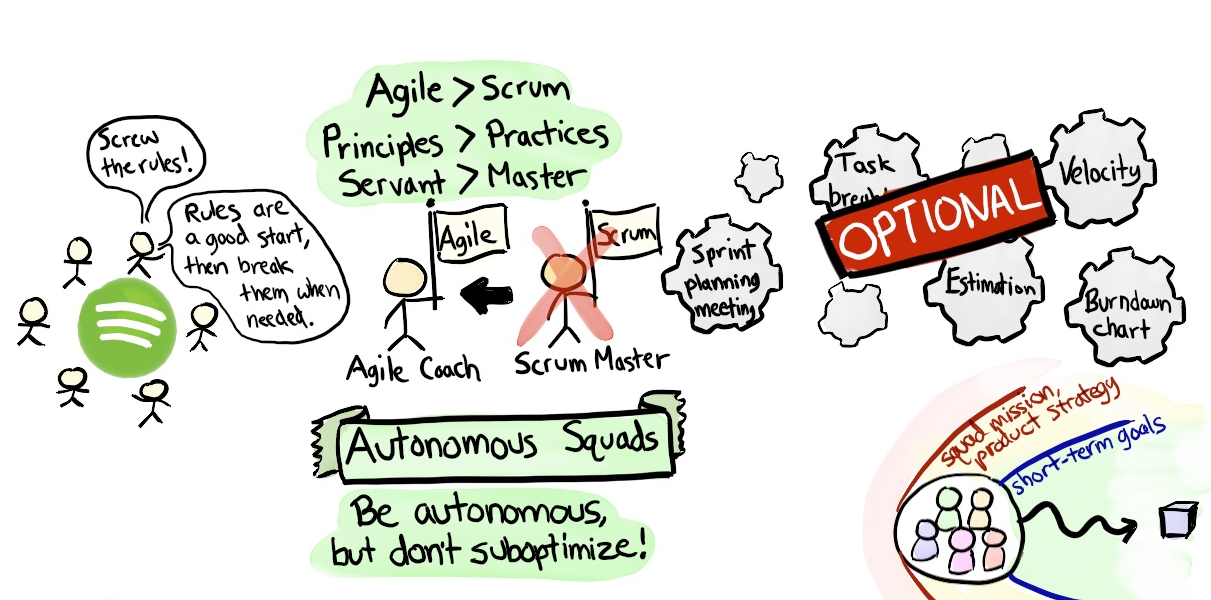
\includegraphics[width=95mm]{./images_spotify/agile_scrum}
\end{center}

Dès ses débuts, Spotify a mis en place une organisation en équipes Scrum, cependant avec la croissance de l'entreprise et la multiplication des équipes, les procédures de Scrum se sont mises à ralentir les équipes.

Partant de l'idée que \textbf{les principes de l'agilité sont plus importants que les pratiques}, les procédures Scrum sont devenues optionnelles et l'organisation des équipes a été chamboulée. Les Scrum Masters sont devenus des coachs Agiles et les équipes Scrum ont été réorganisées en \textbf{Escouades Autonomes}.

Ces escouades sont des équipes \textbf{auto-organisées} --- elles décident de leur organisation interne, de ce qu'elles vont réaliser et de la manière de le réaliser---, \textbf{autonomes et transverses} ---elles sont capables de réaliser une fonctionnalité du début à la fin : conception, développement, tests, déploiement et maintenance--- de moins de huit personnes ayant \textbf{un objectif à long-terme} ---tel que « Faire de Spotify le meilleur endroit pour écouter de la musique » ou « Fournir une infrastructure pour faire du test AB ».

Afin que ces équipes autonomes restent cohérente avec la stratégie de l'entreprise, \textbf{elles sont « alignées » avec la stratégie produit, les priorités de l’entreprise et les autres escouades avec des objectifs à court-terme} négociés tous les trimestres avec leurs supérieurs.

\vspace{5mm}

Pour la direction de Spotify, l'autonomie est extrêmement importante puisqu'ils considèrent qu'elle permet de motiver les employés et que \textbf{des employés motivés construisent de meilleures choses}.

De plus, l'organisation en équipes autonomes réalisant toutes les étapes d'un projet \textbf{permet d'être rapides} en laissant les décisions avoir lieu localement dans l'escouade et de diminuer les transferts de responsabilités à d’autres équipes ---comme lors d'un déploiement réalisé par une autre équipe---, l’attente ou les réunions inter-équipes permettant une mise à l’échelle sans problèmes de dépendances ou de coordination.

Ceci est reflété dans l'architecture de Spotify, organisée en une centaine de micro-services spécialisés, découplés, codés et développés indépendamment. Chacun de ces systèmes appartient à une équipe ---qui en a donc fait la conception, le développement, le déploiement et qui en effectue la maintenance--- et ils sont open-sourcés au sein de Spotify, permettant ainsi à une escouade de soumettre des modifications sur le système d’une autre escouade si cette dernière n’en a pas les capacités. Encore une fois, \textbf{on ne perd pas de temps à attendre que les équipes se coordonnent}.

\newpage

\begin{center}
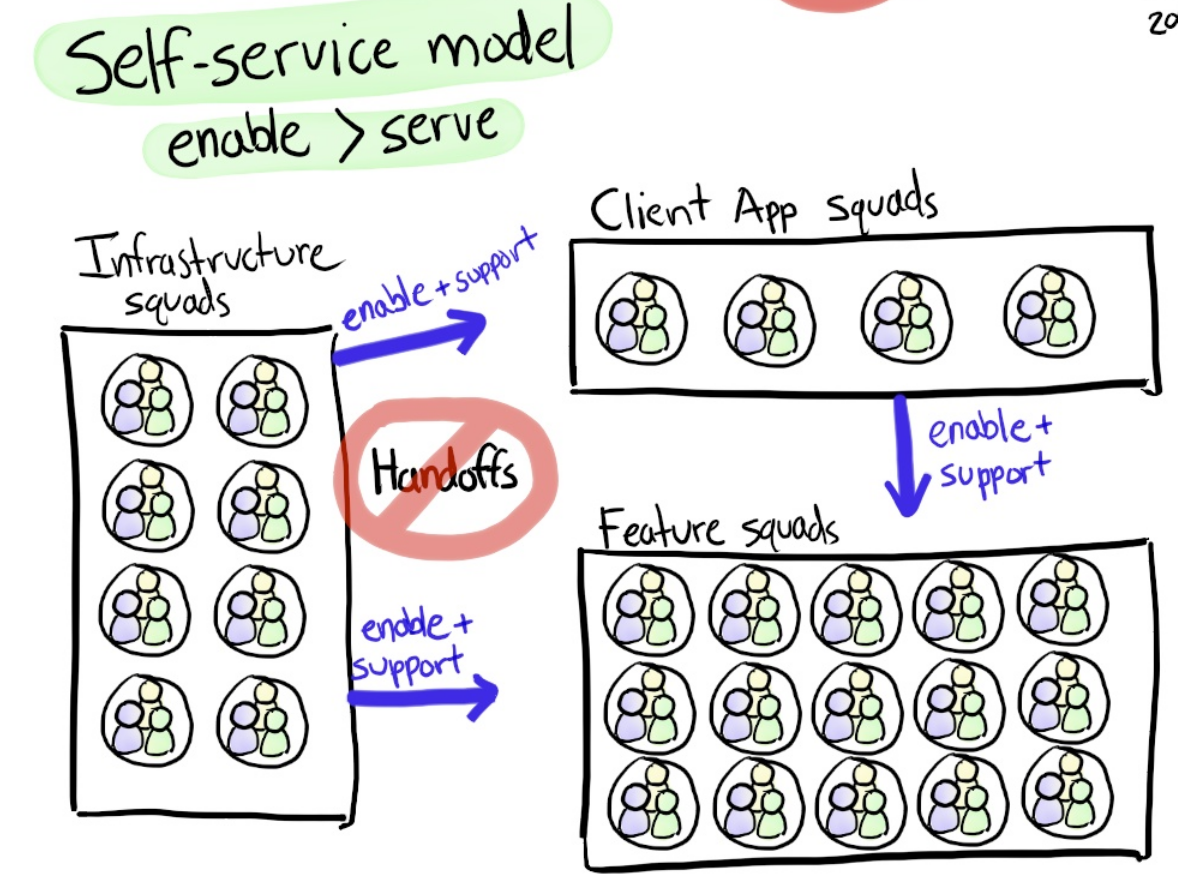
\includegraphics[width=95mm]{./images_spotify/image03}
\end{center}

Ce modèle de « self-service » est aussi appliqué dans les mises en production des fonctionnalités, puisque les escouades sont regroupées en trois types : les escouades s'occupant des clients, les escouades infrastructure et les escouades créant les fonctionnalités.

Le rôle des \textbf{escouades fonctionnalité} est de développer et maintenir toutes les fonctionnalités qu'ils ont à charge (par exemple la recherche de morceaux) sur toutes les plate-formes.

Les \textbf{escouades infrastructure} ont pour objectif de rendre les autres escouades plus efficaces dans leurs mises en production en fournissant des routines et des outils pour la livraison continue, les tests AB et le monitoring.

Les \textbf{escouades clients} quant à elles gèrent un des clients (bureau, web, iOS, Android, etc.) et s'attellent à rendre le déploiement par les autres escouades de nouvelles fonctionnalités au sein de leur client le plus facilement possible.

\newpage

\begin{center}
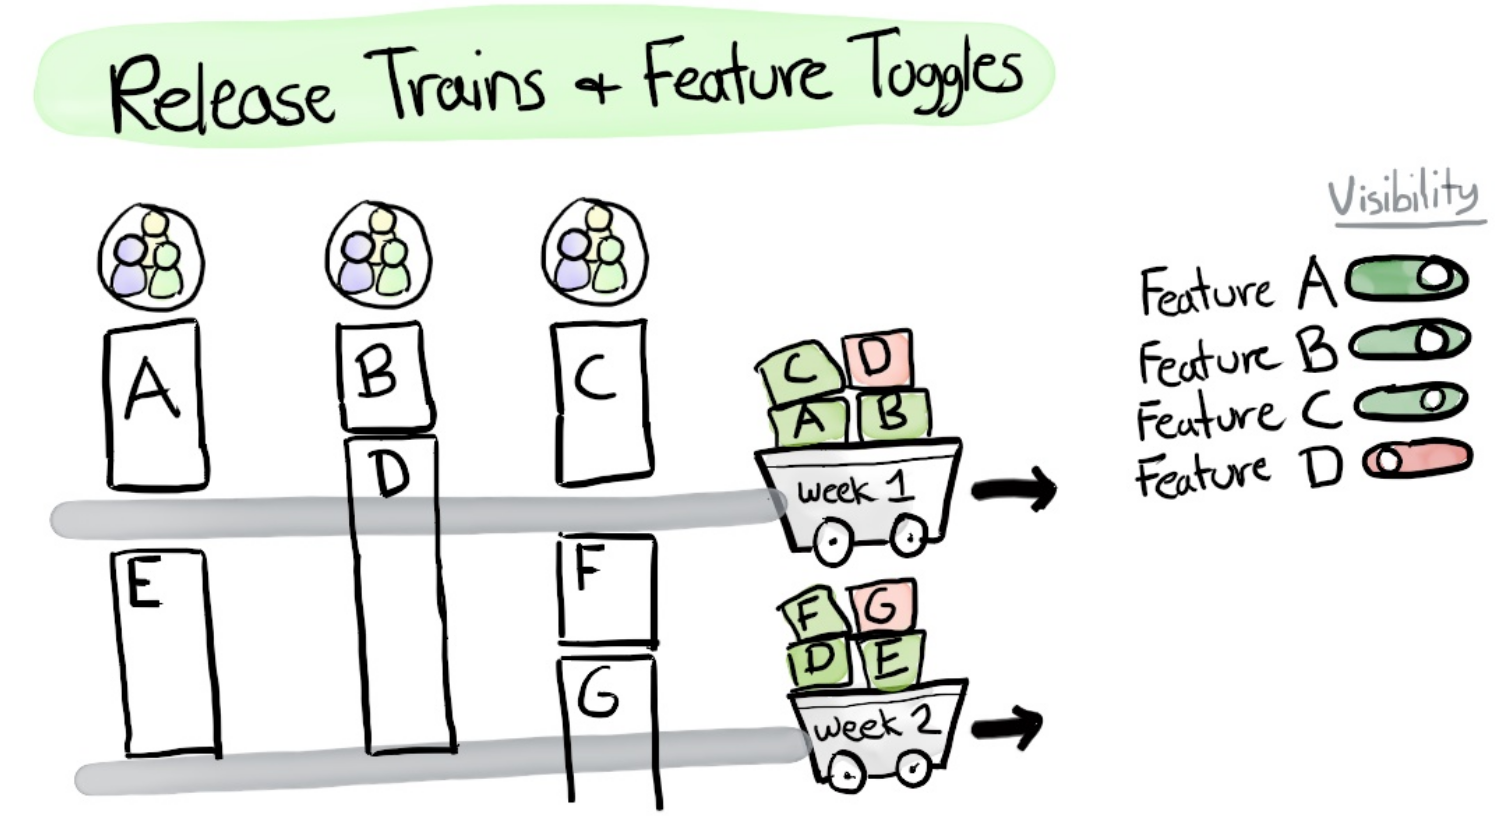
\includegraphics[width=95mm]{./images_spotify/image08}
\end{center}

Ainsi \textbf{Spotify s'efforce de sortir de nouvelles fonctionnalités régulièrement} avec des cycles de release allant de une à trois semaines, et ce même si elles ne sont pas terminées. En effet, chaque fonctionnalité terminées ou en cours de développement est mise en production lorsque le « release train » passe à la fin d'un cycle et les fonctionnalités qui ne sont pas terminées sont masquées avec un « feature toggle ». Ces feature toggle ont plusieurs rôles : masquer les fonctionnalités en cours de développement, tester de nouvelles fonctionnalités en les déployant graduellement aux utilisateurs et masquer des fonctionnalités présentant des erreurs avant qu'elles n'impactent trop d'utilisateurs.

L'architecture découplée et les feature toggles sont importantes dans le processus de création, puisqu'elles permettent de mettre en place \textbf{un environnement dans lequel les développeurs peuvent expérimenter tout en ayant un impact limité en cas d'erreur}. Cet environnement permet également d'encourager les équipes à réaliser plusieurs petites expérimentations et d'en apprendre rapidement, évitant de perdre du temps à prévoir et contrôler les risques en avance.

\newpage

\begin{center}
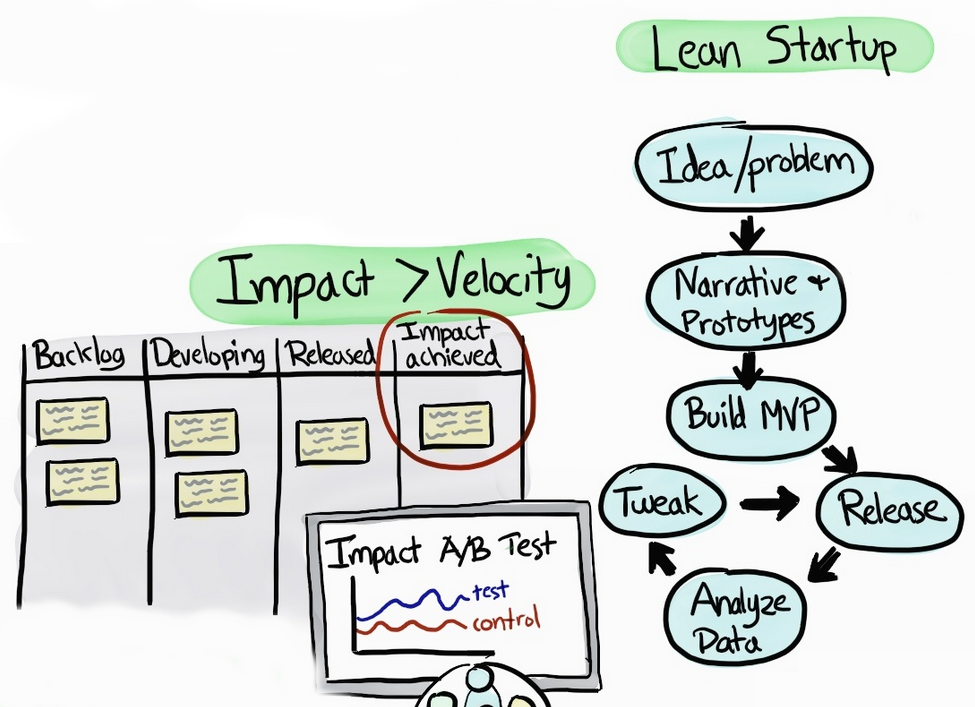
\includegraphics[width=95mm]{./images_spotify/image04}
\end{center}

Le processus de création de fonctionnalité est d'ailleurs \textbf{fondée sur l'expérimentation} : après avoir émit une hypothèse, l'escouade réalise des narratives, des études d'impact puis divers prototypes qui sont testés afin de savoir si les utilisateurs apprécieront la fonctionnalité.

Une fois que l'escouade est confiante dans son idée, elle réalise d’un produit minimum viable qui réalise la narrative mais qui est loin d’être complet. Ce produit minimum viable est par la suite déployé en production et l'escouade réalise des tests A/B afin de tester leur hypothèse. Ces tests sont analysés et la fonctionnalité est ajustée jusqu'à ce que l'impact désiré soit atteint. La fonctionnalité est enfin déployée graduellement au reste des utilisateurs et améliorée par la suite. 

\vspace{5mm}

Il y a une véritable \textbf{culture d'amélioration continue} au sein de Spotify, par le biais de post-mortem et de rétrospectives régulières, mais aussi la mise en place de communautés : 

Chaque employé peut rejoindre une « \textbf{guilde} », une communauté réunissant tous les employés ayant un centre d'intérêt commun tel que le leadership, le  développement web et la livraison continue. Ces guildes sont des lieux d'échanges d'expériences et de bonnes pratiques.

Spotify s'est aperçu qu'\textbf{une organisation autour de communautés fortes permet de se passer d'une structure informelle et volatile} : les escouades sont regroupées en \textbf{tribus} et chaque membre d'une escouade fait partie d'un « \textbf{chapter} », une communauté centrée autour d'une compétence (assistance qualité, coaching agile, développement web, etc.) avec un leader qui coache, mentore ses membres ; leur permettant à l'occasion de changer d'escouade au sein d'une même tribu sans changer de manager.

\section{Netflix : la culture de l'excellence }

\textit{Toutes les informations de cette section proviennent de la présentation de Reed Hastings nommée \texttt{Culture}\supercite{NetflixCultureBook} et de l'article de presse \texttt{How Netflix Reinvented HR}\supercite{NetflixReinventedHR} de Patty McCord, principale investigatrice de la culture d'entreprise de Netflix de 1998 à 2012.} 

\vspace{5mm}

En 2001, l'explosion de la bulle Internet et les attentats du 11 Septembre retardent l'introduction en bourse de Netflix, \textbf{obligeant l'entreprise à se séparer d'un tiers de ses employés}. Quelques mois plus tard en 2002, suite à la popularité des lecteurs DVD durant les fêtes, les services de location de DVD doivent faire face à une demande grandissante ; et \textbf{Netflix se retrouve soudainement avec une charge de travail supplémentaire avec un tiers de ses employés en moins}.

\vspace{5mm}

C'est dans ce contexte que deux conversations vont marquer l'esprit de Patty McCord et définir \textit{la culture Netflix} :

La première est avec un ingénieur qui, suite aux licenciements, se retrouve seul dans son équipe. Il explique que bien qu'il doive travailler plus longtemps, il n'a jamais autant bien travaillé : \textbf{les trois employés qui étaient sous sa responsabilité étaient des employés moyens avec lesquels il perdait beaucoup trop de temps à micro-manager et à corriger leurs erreurs}.

La seconde a lieu avec lieu avec une comptable dont \textbf{les compétences n'étaient plus en adéquation avec les besoins de l'entreprise} après son introduction en bourse. Après lui avoir expliqué qu'ils devaient se séparer d'elle malgré sa longue expérience et sa loyauté envers l'entreprise, l'employée se montre compréhensive et considère le licenciement comme l'occasion de changer de carrière.

\vspace{5mm}

Patty McCord retiendra deux choses de ces entretiens : d'une part que \textbf{des employés « moyens » peuvent freiner les autres}, et d'autre part qu'\textbf{il ne faut pas avoir peur de se séparer d'un employé si il n'est plus indispensable} à l'entreprise. Suite à ça, Netflix va se mettre à \textbf{chercher des employés excellents} et encourager ceux qui ne le sont pas à partir avec des primes de départ généreuses.

Au fil des années, la culture d'entreprise de Netflix s'est articulée afin de permettre d'atteindre l'excellence tant recherchée. 

\vspace{5mm}

Cette excellence est avant tout définie par des \textbf{comportements et compétences promues par Netflix} et recherchées lors des candidatures et des promotions : une capacité de jugement qui soit sage et pragmatique ; de bonnes capacités de communication ; la recherche des meilleurs résultats ; un désir d'apprendre rapidement, de comprendre la stratégie, le marché, les clients et les fournisseurs de l’entreprise ; la création de nouvelles idées innovantes ; la passion, l'honnêteté, la loyauté, le courage et l'altruisme.

Netflix recherche également des employés qui soient \textbf{autonomes et responsables, capables de se discipliner, de s'améliorer, de se motiver et de se comporter en leader}. L'objectif n'est pas seulement de s'entourer des meilleurs talents, mais de \textbf{pouvoir faire fonctionner l’entreprise informellement grâce à l'auto-discipline de chacun}, évitant le chaos induit par la croissance de l'entreprise et l'augmentation de sa complexité tout en permettant une créativité accrue en n'ayant pas à mettre en place des procédures pour tenter de garder le contrôle.

Dans un esprit similaire à celui de Spotify, \textbf{les équipes sont autonomes, transverses et alignées sur les objectifs et la stratégie de l'entreprise}.

\vspace{5mm}

Outre l'autonomie, \textbf{la responsabilité est très valorisée au sein de l'entreprise} : il est attendu des employés qu'ils discutent de leurs problèmes, de leurs compétences et de leurs performances avec leurs supérieurs et collègues, qu'ils gèrent l'argent de Netflix comme le leur, qu'ils gèrent eux-mêmes leurs vacances et qu'ils aient une idée des sources de dépenses et de revenus de l’entreprise afin qu’ils puissent contrôler les dépenses de leurs équipes. 

Brendan Gregg\supercite{WorkingAtNetflix}, ingénieur chez Netflix, considère que cette \textbf{culture de « liberté et responsabilité »} invite les ingénieurs à découvrir et \textbf{proposer de nouvelles solutions, technologies et projets risqués}, pour peu qu'ils soient pertinents et argumentés. 

\section{SpaceX \& Tesla Motors : le culte d'Elon Musk}

\textit{L'essentiel des informations de cette section (ainsi que toutes les autres sections concernant SpaceX et Tesla Motors) proviennent de la biographie \texttt{Elon Musk: Tesla, SpaceX, and the Quest for a Fantastic Future}\supercite{ElonMuskBiography} d'Ashlee Vance, journaliste chez Bloomberg. Les informations restantes proviennent des articles de presse cités dans cette section.} 

\vspace{5mm}

Bien qu'Elon Musk n'ait pas techniquement fondé Tesla Motors, \textbf{il a néanmoins fortement influencé la culture de l'entreprise} dès ses débuts : il a profité de sa popularité auprès de la presse pour être le visage de l'entreprise et il a eu une influence forte sur sa stratégie grâce à son statut d'actionnaire principal.

Son influence sur l'entreprise a par la suite augmenté après que le conseil d'administration ait remercié Eberhard et nommé Ze'ev Drori puis Elon Musk président de Tesla Motors en Octobre 2008\supercite{MuskTeslaCEO}.

Alors qu'aux débuts de SpaceX et Tesla il ait voulu appliquer sa vision jusqu'alors limitée aux projets logiciels (notamment son expérience chez \textit{Zip2} et \textit{X.com}), il a dû réviser ses méthodes de management et les adapter aux contraintes de la production de biens physiques.

\vspace{5mm}

Parmi les méthodes apportées du monde des start-ups, les \textbf{itérations rapides} étaient présentes dès les débuts de la conception du Roadster et de Falcon 1. L'un des principes clés chez Tesla et SpaceX est de pouvoir \textbf{rencontrer rapidement un problème afin de le diagnostiquer et le résoudre le plus tôt possible}.

Pour cela les deux entreprises ont \textbf{massivement recourt aux simulations} : non seulement elles étaient indispensables aux débuts faute de moyens financiers pour réaliser plusieurs prototypes pour les tests, mais elles permettent également de reproduire et corriger des anomalies très rapidement.

\textbf{L'exemple parfait réside dans les bancs de test de SpaceX} sur lequels se trouvent des répliques de l'ensemble des systèmes des fusées Falcon : dès lors qu'une anomalie est détectée sur la fusée durant le lancement, les ingénieurs peuvent la reproduire, réaliser des corrections, les tester sur la réplique puis les envoyer sur la fusée sur le pas de tir \textbf{en seulement quelques heures}, là où la NASA aurait annulé le tir et réalisé un nouvel essai trois semaines plus tard.

\vspace{5mm}

Comme le montre ce recourt aux simulations, une véritable \textbf{chasse au gâchis} a été entreprise par Elon Musk au sein des deux entreprises : \textbf{toute dépense de plus de 10 000 dollars doit être approuvée par ses soins} ---après tout, c'est sa fortune qui est dépensée--- et un \textbf{maximum des pièces sont réalisées en interne}, et ce pour plusieurs raisons.

Tout d'abord parce qu'il \textbf{considère la dépendance aux sous-traitants comme une faiblesse} : non seulement l'entreprise peut se retrouver en difficulté si un sous-traitant les abandonne ou fait faillite, mais \textbf{passer par des intermédiaires fait perdre du temps}.

La seconde raison réside dans les \textbf{besoins spécifiques des deux entreprises} : beaucoup de pièces n'existent pas dans l'industrie ---notamment les moteurs et packs de batteries--- \textbf{ou sont proposées à des tarifs excessifs}, comme celles provenant de l'industrie aérospatiale.

À plusieurs reprises SpaceX a conçu et réalisé des pièces et systèmes \textbf{moins chers, plus compacts et tout aussi performants que leurs équivalents de l'industrie spatiale}, permettant de réaliser de nombreuses économies. Par exemple, les systèmes informatiques des capsules Dragon et des fusées Falcon 9 coûtent près de 10 000 dollars à réaliser contre près de 10 millions de dollars chez la concurrence, tout en réalisant un gain d'espace conséquent dans la capsule Dragon.

Ainsi chez SpaceX \textbf{80 à 90\% des pièces sont réalisées en interne}, là où United Launch Alliance se présente comme un créateur d’emplois en dépendant de près de 1200 fournisseurs différents ; tandis que \textbf{Tesla produit l'intégralité ses Model S et X en trois à cinq jours}.

\vspace{5mm}

SpaceX et Tesla Motors sont dans une \textbf{stratégie d'amélioration continue} : leurs \textbf{usines sont continuellement optimisées} et \textbf{mélangent intelligemment robots et ouvriers} de différents corps de métier. Les premiers ne sont utilisés que pour les tâches très répétitives ou nécessitant une grande précision tandis que les seconds sont employés pour les tâches où l'intelligence humaine est indispensable\supercite{TeslaFactoryPart2}.

Le mélange des corps de métier est une pierre angulaire de SpaceX où \textbf{les ingénieurs côtoient quotidiennement les ouvriers}, les guident et suivent leurs avancées.

\vspace{5mm}

Musk a également poussé les entreprises à utiliser des \textbf{techniques novatrices} telles que le \textit{soudage par friction malaxage}. Alors que les principaux constructeurs de fusées l'évitent au profit des soudures traditionnelles à cause des faiblesses pouvant être introduites par cette technique, Musk a insisté afin que cette technique soit perfectionnée et utilisée au sein de SpaceX. 

Le pari en valait la peine puisque la technique leur a permis d'utiliser des alliages plus légers et de se passer de rivets et de structures de soutiens, résultant en des \textbf{gains de poids conséquents}. La méthode a depuis été transférée à Tesla et commence à être \textbf{imitée par ses concurrents} ---notamment \textit{Blue Origin} qui a débauché l'un des ingénieurs ayant mis au point la technique.

\vspace{5mm}

Une chose que Musk a cependant gardé intact de l'esprit start-up de ses débuts est la \textbf{recherche continue des meilleurs talents}. Pour cela ses entreprises n'hésitent pas à approcher les universités afin de recruter directement les étudiants les plus brillants ou encore à inviter certains participants d'une convention à un entretien privé dans un bar ou restaurant proche.

Musk recherche des\textbf{ esprits brillants et passionnés} capables de résoudre des problèmes concrets et \textbf{ayant une expérience manuelle} telle que la participation à un concours de robotique ou la construction d'un véhicule électrique sur leur temps libre.

Les premiers entretiens se concentrent sur le parcours et la motivation des candidats tandis que les suivants se déroulent avec les managers et les futurs collègues afin de s'assurer qu'il s'intégrera correctement à l'équipe. Pour les postes les plus techniques il leur sera demandé de \textbf{diagnostiquer des problèmes concrets et de trouver une solution}, de réaliser un programme de plusieurs milliers de lignes en quelques heures ou encore d'analyser des données sans instructions.

Pour SpaceX ces postes à haut niveau doivent passer une étape supplémentaire : ils doivent \textbf{rédiger une dissertation sur leurs motivations à destination d'Elon Musk}, qui les conviera à un entretien final. Durant cet entretien Musk a pour habitude de poser une énigme aux candidats. L'exactitude de la réponse importe peu, il \textbf{s'intéresse avant tout au raisonnement} qu'ont eu les candidats.

\vspace{5mm}

Avec des employés si motivés et talentueux, les entreprises se permettent de \textbf{maximiser le pouvoir des individus}. Elles partent du principe qu'un individu prêt à abattre une masse incroyable de travail peut réaliser plus de travail qu'un groupe, puisqu'il ne perd pas de temps à être interrompu, à obtenir le consensus ou à organiser des réunions.

Cependant \textbf{ce rythme de travail est loin de convenir à tous} ---les ingénieurs travaillent souvent près de douze heures par jour---, d'autant plus que les \textbf{ingénieurs sont laissés en autonomie} et que Musk attend d'eux qu'ils soient capable d'abattre autant de travail que lui ---il est réputé pour avoir une endurance sans commune mesure et d'être capable de travailler plus de trois jours de suite sans jamais s'arrêter ni dormir---, amenant certains à quitter l'entreprise quelques semaines après leur embauche. 

\chapter{Des stratégies qui paient et des challenges à venir}

En supplément du Chapitre 3, il est à remarquer que les quatre entreprises étudiées ont suivi la \textit{Stratégie Océan Bleu}\supercite{BlueOceanStrategy}.

Dans cet ouvrage écrit par deux chercheurs de l'\textit{INSEAD}, le marché se compose de deux ensembles d'océans : les \textbf{océans rouges}, la partie qui est déjà exploitée par des entreprises ; et les \textbf{océans bleus}, la partie du marché qui est encore vierge de toute activité et concurrence.

L'ouvrage préconise aux entreprises de \textbf{conquérir ces océans bleus incontestés} en y créant une demande et de \textbf{profiter de l'absence de concurrence établie pour croître rapidement}.

\vspace{5mm}

Ainsi SpaceX s'est d'abord concentré sur le lancement de petits satellites avant de s'atteler aux marchés plus important, 

Tesla Motors a créé une voiture entièrement électrique à une époque où les constructeurs se limitaient aux véhicules hybrides, 

Spotify a été le premier service d'écoute de musique à la demande crédible\footnote{De nombreuses radios en ligne (dont \textit{Pandora}) et \textit{Blogmusik} (l'ancêtre de \textit{Deezer}) existaient déjà lors du lancement de la bêta de Spotify en 2007. Bien que Blogmusik est considéré comme le premier service d'écoute de musique à la demande, il opérait en toute illégalité.} et fut lancé alors que \textit{The Pirate Bay} était à son apogée,

et Netflix a été le premier sur la location de DVD et la vidéo à la demande illimitée en Amérique du Nord.

\vspace{5mm}

D'autant la Stratégie de l'Océan Bleu est extrêmement pratique pour s'insérer dans un marché et croître rapidement, il faut savoir adopter une stratégie à plus long terme afin de pouvoir \textbf{continuer à croître} et \textbf{entrer en compétition avec les concurrents établis}.

\vspace{5mm}

Après que SpaceX ait pu obtenir des \textbf{revenus réguliers grâce à ses nombreux lancements}, l'entreprise a pu sereinement lancer le développement de la fusée Falcon 9 et de la capsule Dragon. Ces deux développements leur ont alors permis d'ouvrir les portes des contrats gouvernementaux avec la NASA pour \textbf{ravitailler la Station Spatiale Internationale} et de \textbf{rentrer en compétition} directe avec \textit{Arianespace} et \textit{RSC Energia} qui avaient récupéré la majeure partie du marché après l'abandon du programme \textit{Space Shuttle}.

Arianespace est alors \textbf{mis en difficulté} puisqu'un lancement d'Ariane 5 coûte entre 165 et 220 millions de dollars\supercite{Ariane5Cost} tandis qu'un lancement de Falcon 9 ne coûte que 62 millions de dollars\supercite{FalconCost}. 

SpaceX souhaite \textbf{continuer sa conquête du marché} avec sa fusée \textbf{Falcon Heavy} qui dispose d'une capacité similaire à Ariane 5 pour un coût de lancement estimé à 90 millions de dollars. Alors que les premiers essais de Falcon Heavy vont commencer cet hiver\supercite{FalconHeavyFirstLaunch}, \textbf{Ariane 6 ne sera pas opérationnelle avant 2020}\supercite{Ariane6Debuts}. \textbf{Arianespace espère redevenir compétitif} avec son coût de lancement entre 60 et 115 millions d'euros (selon la configuration et les charges)\supercite{Ariane6Cost}.

Avec sa \textbf{capsule habitée Dragon 2} en développement, l'entreprise souhaite également \textbf{récupérer le marché du transport d'astronautes} pour la Station Spatiale Internationale qui dépend actuellement des capsules Soyouz ; et l'envoyer \textbf{effectuer ses premières missions sur Mars} d'ici la fin de la décennie\supercite{ElonMuskMars2020}.

\vspace{5mm}

Pour sa part Tesla Motors \textbf{a abordé le marché par le haut} en débutant avec des modèles très haut de gamme puis en descendant de gamme \textbf{à fur et à mesure que la technologie est maîtrisée et abordable}. L'entreprise suit scrupuleusement son « plan secret »\supercite{TeslaSecretMasterPlan} depuis dix ans : tandis que le Roadster était commercialisé à 90 000 dollars, les très luxueux modèles S et X commencent à 60 000 dollars et 83 000 dollars respectivement et \textbf{le futur Model 3 devrait débuter à 35 000 dollars}.

Ce Model 3 va s'avérer être \textbf{le modèle de la maturité} pour Tesla : l'entreprise devra produire plusieurs centaines de milliers d'exemplaire d'ici 2017, soit \textbf{bien plus que sa capacité de production actuelle} de 107 000 exemplaires en 2015\supercite{Tesla2015FullYearUpdate}. Cette quantité d'exemplaire va également nécessiter une \textbf{quantité de batteries sans précédent} puisque selon les dires de Musk\supercite{Model3Unveil} le double de la production actuelle de batteries sera nécessaire.

Pour y remédier, Tesla Motors a ouvert une seconde usine en Europe à \textit{Tilbourg} aux Pays-Bas en 2013\supercite{TeslaTilburgFactory} et sa \textbf{Gigafactory}, une gigantesque usine de batteries recouverte de panneaux solaires au plein milieu du Nevada, fondée en collaboration avec \textit{Panasonic}. \textbf{Capable de produire 35 millions de mWh} de batteries, elle devrait commencer la production dès 2017\supercite{Gigafactory}.

Enfin, Tesla \textbf{doit parvenir à devenir profitable} puisqu'en 2015 l'entreprise perdait encore 4000 dollars sur chaque Model S produite\supercite{TeslaLoses}.

\vspace{5mm}

Bien que son énorme catalogue et sa facilité d'utilisation aient participé au succès de Spotify auprès des utilisateurs, \textbf{il lui faut rester attrayant auprès des maisons de disques}. D'un côté se trouvent les cinq principales maisons de disques qui possèdent 18\% des parts de l'entreprise\supercite{LabelsOwnSpotify}. De l'autre se trouvent les labels indépendants qui \textbf{suspectent que leurs revenus soient inférieurs} à ceux des labels actionnaires\supercite{SpotifyBloomberg}.

Pour attirer ces derniers, Spotify leur \textbf{promet des revenus sur le long-termes} puisqu'ils sont récurrents et générés à chaque écoute, là où un album ne rapporte que lors de sa vente. De plus Spotify leur \textbf{fourni de nombreuses informations sur leur audience}, permettant par exemple de déterminer les lieux idéaux pour la tournée d'un groupe.

L'avenir de Spotify s'annonce difficile puisque l'entreprise \textbf{peine à être rentable} à cause des sommes astronomiques qu'elle doit reverser aux labels\supercite{SpotifyChiffres2015}. De plus l'arrivée d'Apple sur le marché risque de ne pas arranger ses affaires puisque son service \textbf{Apple Music a recruté 15 millions d'abonnés en tout juste un an}\supercite{AppleMusic15Million} tandis que Spotify n'en a recruté que 10 millions sur la même période.

\vspace{5mm}

Alors que Netflix a su attirer ses premiers utilisateurs grâce à son catalogue, \textbf{il a fallu qu'il puisse les retenir}, et par extension, garder ses revenus. Pour cela\textbf{ Netflix a su se rendre indispensable grâce à son système de recommandations} intégré à son service de location de DVD puis à son service de vidéo à la demande.

À partir de l'analyse des films et séries par des employés indépendants et l'\textbf{analyse des habitudes de visionnage} de ses utilisateurs, Netflix est capable d'effectuer des recommandations en fonction de l'historique de l'utilisateur et du contexte comme l'heure de la journée\supercite{NetflixAlgorithm}.

Mais plus encore, Netflix a su tirer profit de ces analyses afin de \textbf{commander des séries exclusives et acclamées par la critique capables d'attirer de nouveaux utilisateurs}. On peut citer des séries telles que \textit{House of Cards}\supercite{HoCAwards}, \textit{Orange Is The New Black}\supercite{OitNBAwards} et \textit{Narcos}\supercite{NarcosAwards}. Les saisons de ces séries ont également la particularité, contrairement au modèle de diffusion classique, d'être disponibles dans leur intégralité, laissant le choix aux utilisateurs de les regarder au rythme qu'ils souhaitent.

\textbf{L'objectif affiché depuis quelques années est désormais le développement à l'international} : le service de vidéo à la demande a commencé sa conquête de l'Europe en 2012\supercite{NetflixEurope} et est désormais disponible dans le monde entier depuis le mois de Janvier\supercite{NetflixAvailableWorld}. Enfin, Netflix compte produire du contenu local tels que la série \textit{Marseille} afin d'attirer les clients de ces nouveaux pays\supercite{NetflixNumerama}.

\vspace{5mm}

En conclusion ces entreprises \textbf{ont su tirer profit de nouveaux espaces de marché avec des produits novateurs, des stratégies en rupture et des cultures d'entreprise fortes} leur offrant rapidité, réactivité et agilité \textbf{afin de croître rapidement et de s'attaquer par la suite aux géants}.

Bien que ce mémoire prenne pour exemples Netflix, Spotify, SpaceX et Tesla Motors, ce ne sont pas les seules entreprises qui ont usé d'une stratégie et d'une culture d'entreprise similaires. Parmi les exemples les plus parlants, on peut citer \textbf{Zappos}.

\vspace{5mm}

Zappos est un \textbf{service de vente de chaussures en ligne créé en 1998} à partir du constat simple de l'entrepreneur \textit{Nick Swinmurn} : le marché des chaussures représente près de 40 milliards de dollars et il souhaite avoir sa part du marché.

Cependant \textbf{personne ne pense que les clients sont prêts à acheter des chaussures sans les essayer}. Beaucoup d'investisseurs trouveront cette idée risquée, jusqu'à ce qu'il rencontre \textit{Tony Hsieh}, convaincu par les 5\% de parts de marché représentés par la vente par correspondance.

Outre la création du marché de la vente de chaussures en ligne, Zappos \textbf{définira sa culture autour du service rendu et de la satisfaction du client}, imposant à ses employés de faire tout ce qui en leur pouvoir pour résoudre les problèmes de leurs clients, quitte à les diriger vers des sites concurrents en cas de rupture de stock.

Désormais une filiale d'\textit{Amazon} suite à son rachat en 2009 pour 1,2 milliards de dollars et \textbf{réalisant près de 2 milliards de dollars de bénéfices par an}\supercite{ZapposForbes} ; l'entreprise \textbf{se dirige vers une organisation holacratique}, une structure horizontale et auto-organisée \textbf{considérée par Tony Hsieh comme l'avenir des organisations d'entreprises.}

\newpage
\nocite{SpaceXFirstISS, IFPI2011Report, SpotifyBloomberg, SpotifyNewYorker}
\printbibliography

\end{document}